\section{RATIONALE ON THE COMBINATION BETWEEN VISUALIZATION AND DATA CLUSTERING}\label{sec:rationale}%

In many cases, the analyst, with some knowledge of a system, can perform an analysis of the results and create a concise final model. However, especially for complex systems, it is necessary to use strategies for interpretation of results. Such strategies involve the observation of repeated patterns and identification of architectural violations in the source code.

In general, automatic architecture reconstruction methods, such as clustering technique, has the advantage to produce different models for a single software system in a short period of time. Such models can be constructed differently by changing configuration settings on clustering algorithm used during the process. Through the analysis of different models it is possible to identify patterns that recur frequently in the results.

However, when the idea is not clear of how the system structure is composed, the various models produced by clustering process can not help to understand complex software \cite{craft}, since the results show a high level view of the architecture. In this sense, the use of software visualization technique permit an observation of different outcomes on a low level of abstraction. By means of interactive operations in the models produced by the visualization software, it is possible to decompose components of the system in more detailed representations. Thus, allowing the observation of concepts as part of the architecture in greater depth.

In this context, linking the models produced by the clustering process with the model produced by the software visualization process, it is possible to get different representations of the system to form a final model with greater precision. For example, take into account the results shown in Figure \ref{exemplo_comparacao_modelos}. Assuming that the process of obtaining architecture models recovered four different results, through the use of software visualization technique and clustering algorithms. Each model features 9 entities, namely: \{1,2,3,4,5,6,7,8,9\}. By performing a count of the grouped entities it is  possible to obtain the ratio of how many times the entity was classified similarly to the other. The result of this count is observed in Table \ref{ocorrencias_1}.

\begin{table}[]
	\centering
	\caption{Occurrences of entities in the results.}
	\label{ocorrencias_1}
	\begin{tabular}{|cc|}
		\hline
		\multicolumn{1}{|l}{Relation} & \multicolumn{1}{l|}{Occurrence} \\ \hline
		\{1,2,3\}                   & 100\%                           \\
		\{1,2,3,4\}                 & 25\%                            \\
		\{4,5\}                     & 50\%                            \\
		\{4,5,6\}                   & 25\%                            \\
		\{5\}                       & 25\%                            \\
		\{6\}                       & 25\%                            \\
		\{6,7,8,9\}                 & 50\%                            \\
		\{7,8,9\}                   & 100\%                           \\ \hline
	\end{tabular}
\end{table}

By analyzing the results, it is possible to see that the entities \{1,2,3\} can be classified into a single module, since they appear 100\% of the times in the same relation; so do the entities \{7,8,9\}. The entities \{4,5,6\} may be classified as either a single module or each entity may be added to any other adjacent module, since there is no agreement between the results. In these cases, additional analysis must be performed for each entity. This simple example illustrates how to use different results to help the composition of a single final model. In many cases, the aggregation of results provide technical assistance, by highlighting the common patterns. It is possible to gain confidence that agreement across a collection of results can reflect the system structure \cite {craft}.

\begin{figure}[!h]
	\centering
	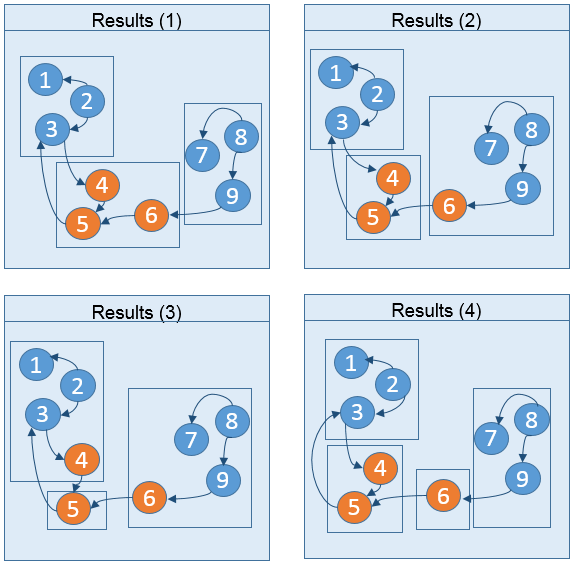
\includegraphics[width=0.43\textwidth]{exemplo_comparacao_modelos_en}
	\caption{Different results for comparison.}
	\label{exemplo_comparacao_modelos}
\end{figure}


However, a more careful analysis of the results, may reveal that other factors may influence the final model produced by clustering and visualization software techniques. A software system throughout its life cycle is susceptible to several changes in its architecture. However, such operations can introduce architectural violations in the code, for example, violation of the layers,  break of abstractions, feature duplication \cite {kazman_view_1998}. In this context, reverse engineering methods are strongly affected by those shortcomings in the system code base \cite {Platenius_2012}.  Such violations should be identified and addressed, so it does not affect the correctness of the final model.

To illustrate a violation on an architecture,  we will use the same results of Figure \ref{exemplo_comparacao_modelos}.  This Figure illustrates a representation of an architecture components through a dependency structure matrix. The figures depicts how the interaction works. The software elements are numbered from 1 to 4, where, for example, the Presentation module (2) requires information from the Visualization module (1). On the other hand, the figures shows also that the Visualization module (1) provides information to the Data module (4).

 \begin{figure}[!h]
 	\centering
 	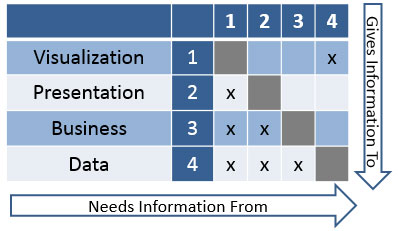
\includegraphics[width=0.42\textwidth]{3_exemploMatrizViolada_en}
 	\caption{DSM representation	of dependences.}
 	\label{3_exemploMatrizViolada}
 \end{figure}
 
 Assuming the entity 4 is wrongly mapped as part of a module. This happens due to a coupling between entities 4 and 5, which illustrates an architecture violation. All results would be classified differently if such violation was removed, as shown in Figure \ref{exemplo_comparacao_modelos2}. The results of the new analysis, taking into account the aggregation of similar entities, can be seen in Table \ref{ocorrencias_2}. Analyzing the results, it is possible to check the impact of the violation. The module containing the first mapping \{1,2,3\} now adds  entity 4, since this set was rated similarly on all results. As for the mapping \{5,6\} there is also a higher chance of being classified in a same module, as it occurs with higher frequency.


\begin{table}[]
	\centering
	\caption{Occurrences of entities between the results after elimination of architectural violation}
	\label{ocorrencias_2}
	\begin{tabular}{|cc|}
		\hline
		\multicolumn{1}{|l}{Relation} & \multicolumn{1}{l|}{Occurrence} \\ \hline
		\{1,2,3,4\}                   	  & 100\%                           \\
		\{5\}                			  & 50\%                            \\
		\{5,6\}                    		  & 50\%                            \\
		\{6\}                 			  & 25\%                            \\
		\{6,7,8,9\}                       & 25\%                            \\
		\{7,8,9\}                         & 100\%                            \\ \hline
	\end{tabular}
\end{table}

\begin{figure}[!h]
	\centering
	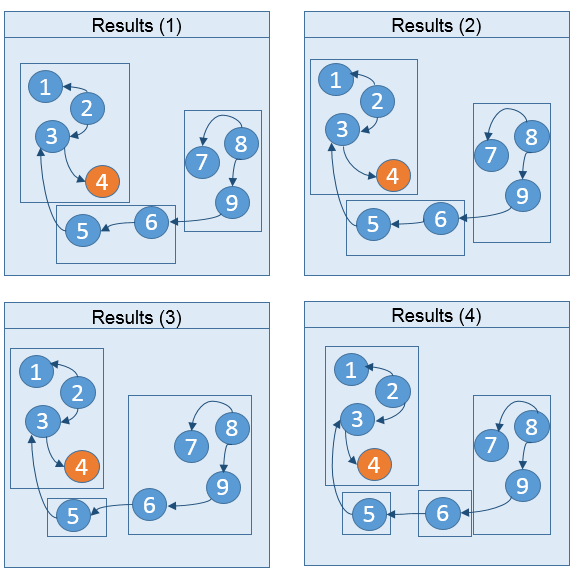
\includegraphics[width=0.43\textwidth]{exemplo_comparacao_modelos_2_en}
	\caption{Eliminating the architectural violation of results.}
	\label{exemplo_comparacao_modelos2}
\end{figure}

Such violations can be found through an analysis of the artifacts produced by software visualization. As an example, take into account the dependency structure matrix shown previously in Figure \ref{3_exemploMatrizViolada}. Through observation of the DSM, it is possible to note a relationship exists between layers, and each layer depends on the upper layers. However, this relationship is violated by layer "Date" (4), since it uses resources of the layer  "View" (1), characterizing an architectural violation. Once the violation is detected, it should be treated as failure and, if necessary, modify the data set for the clustering process, so that the relationship is not considered. Thus, avoiding the production of wrong models that may affect the interpretation of the results.
